\chapter{The Sensory Afferent Database}\label{ch:database}
\graphicspath{{figs/50-database/}}

\section{The Resource}\label{sec:sadb_resource}

The Sensory Afferent Database (SADb) is a curated literature resource for studying sensory feedback in locomotion and posture. It connects papers to afferent classes, experimental preparations, feedback pathways, and computational models. I developed it within the AARL's NeuroNex Communication, Coordination, and Control in Nervous Systems (C3NS) effort and presented the resource at Neuroscience 2023 \citep{bolen_sensory_2023}.

When I began this work, the project lacked a structured resource linking measured afferent properties and feedback pathways to the evidence needed for robot-controller design. Relevant findings were dispersed across species, preparations, tasks, and primary papers. Reviews organized parts of this evidence \citep{van_de_crommert_review_1998, windhorst_muscle_2007, windhorst_spinal_2022}, but selecting a feedback rule still required recovering its experimental conditions and separating measurements from modeling assumptions. I built the SADb to connect those findings to their sources, afferent classes, and pathway roles so that controller choices could be traced to the evidence and remaining unknowns could be identified.

The primary deliverable is a browser application for searching paper records, counting them by selected classifications, and exploring citation neighborhoods (Figure~\ref{fig:sadb_clusters}). Its embedded data support offline use; its separate online-search tab requires a network connection. The distributed snapshot contains 1,393 records: 943 papers and 450 linked model, review, feedback-pathway, and recorder records. Records removed from the working Airtable base remain available in the application as archived records. This separates the collection used for ongoing curation from the broader set of records considered during its assembly. The pivot and citation views operate on papers; the table view searches across record types. For a selected paper, references are the works it cites, whereas citing papers are works that cite it. The citation view distinguishes these directions.

The working base is contained in Airtable, an online database program. Its linked tables organize Papers, Feedback Pathways, Models, and Review Papers. A paper record contains bibliographic information and curation notes: short summaries of its reported mechanism, experimental conditions, and relevance to feedback design. A feedback-pathway record describes a sensory influence on motor control, such as Ib feedback influencing the stance-to-swing transition, and links that description to supporting papers. A model record connects a computational implementation to its source literature; a review record summarizes literature relevant to the collection. Thus, a pathway identifies a mechanism, the linked papers supply its experimental support, and model records identify implementations to examine. These links organize evidence; they do not establish that every relationship has been entered or verified. Paper matching uses DOI where available and normalized titles otherwise. The paper-table view is shown in Appendix~\ref{app:sadb_records} (Figure~\ref{fig:sadb_explorer}).

\begin{figure}[htbp]
\centering
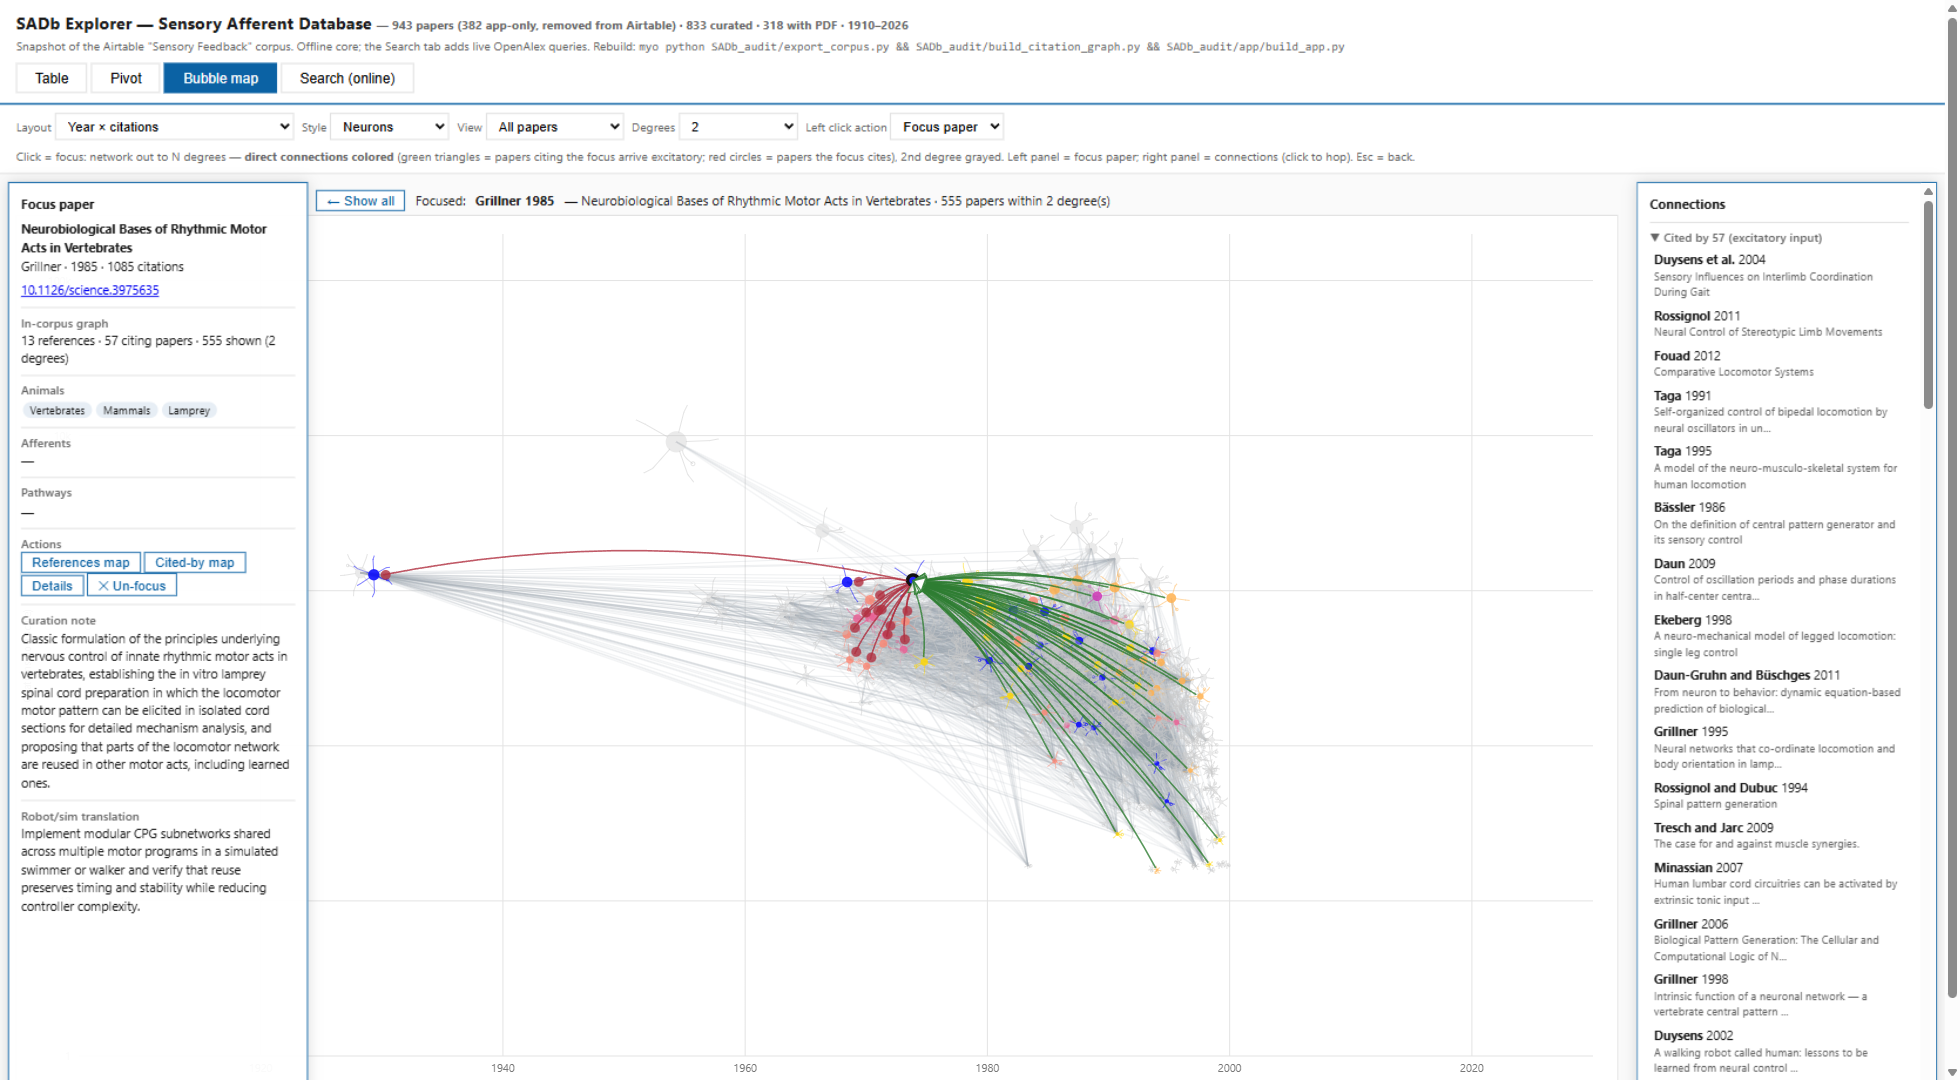
\includegraphics[width=0.94\textwidth]{sadb_clusters_app.png}
\caption[SADb citation-neighborhood view]{Paper-only citation view focused on Grillner (1985). Soma size represents citation count; axes show year and citation count. Triangles mark 57 papers in the corpus that cite Grillner (1985); circles mark 13 papers cited by Grillner (1985). Gray papers connect through one of those neighbors rather than directly to the selected paper. The panels distinguish incoming citations from the selected paper's references.}
\label{fig:sadb_clusters}
\end{figure}

\section{Curation Methods}\label{sec:sadb_methods}

This was a curated research collection, rather than a registered systematic review or an exhaustive search of every relevant publication. The collection began with the libraries used to provide background and understanding for the previous publications on locomotion and postural balance control in the AARL lab. Records were reconciled by DOI and title, then expanded through citation searches. Reviews of spinal and proprioceptive feedback supplied an initial organization of the literature \citep{van_de_crommert_review_1998, windhorst_muscle_2007, windhorst_spinal_2022}. 

Records were retained when they reported measurements from sensory afferents, investigated feedback in locomotion or posture, or modeled a sensory pathway relevant to those tasks. Here, a sensory pathway means the route by which a sensory signal influences neural activity or motor output, such as force feedback from a muscle influencing the transition from stance to swing. Reviews helped organize the subject and locate primary evidence. Duplicate records and material outside this scope were archived. Classification used a consistent set of tags for the experimental preparation and afferent class, allowing papers that used different terminology to be retrieved together. Each mechanism summary was based on the available source text, using the abstract when full text was unavailable.

\subsection{AI-Assisted Triage}\label{sec:sadb_triage}

I evaluated AI-assisted literature identification, summarization, and categorization in work presented at Neuroscience 2024 \citep{bolen_using_2024}. The comparison included ResearchRabbit, Litmaps, txyz, SciSpace, and MirrorThink. Some tools helped identify related papers or summarize straightforward material, but categorization remained inadequate: none received a good rating, and only txyz was rated adequate. Complex models and nuanced physiological findings required substantial human correction. The tools therefore offered limited help with the central curation task of accurately assigning papers to database categories. I retained responsibility for inclusion, classification, and deletion decisions after checking the source.

\section{Coverage and Use}\label{sec:sadb_corpus}

The audited paper set contains 943 records; 561 were retained in the working base. Of those retained papers, 523 have curation notes, 426 have preparation tags, 86 have an afferent classification, and 258 have notes relating their findings to robot or simulation use. These counts describe curation coverage, not the number of independent physiological findings or a measure of their reliability. The more detailed record counts and linked pathway examples are given in Appendix~\ref{app:sadb_records}.

A user of the database can begin with a preparation or afferent class, retrieve the matching papers, and inspect their notes and source links. The pivot view counts papers along two selected dimensions (Figure~\ref{fig:sadb_pivot}); the citation view provides a second route from an anchor paper to related literature (Figure~\ref{fig:sadb_clusters}). These views help locate evidence, while the original experiment determines the conditions under which a finding applies.

\begin{figure}[htbp]
\centering
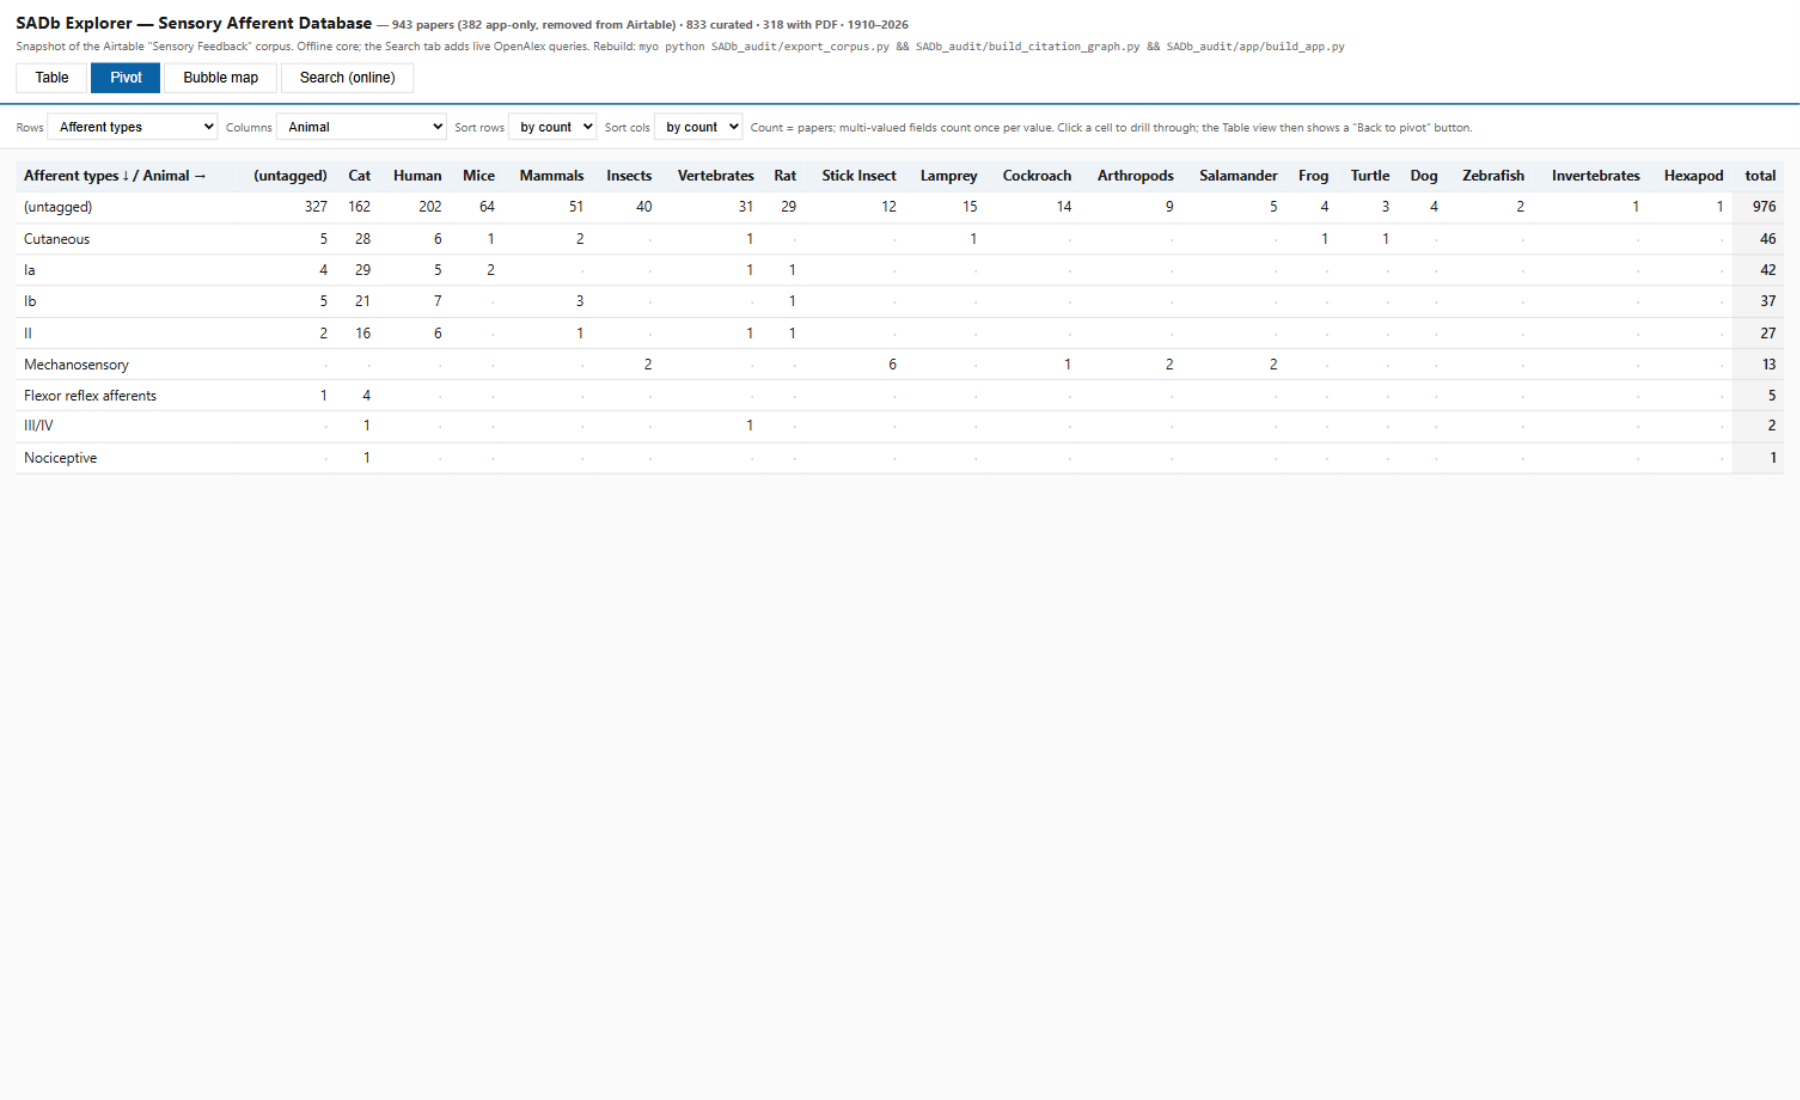
\includegraphics[width=0.96\textwidth,trim=0 610bp 980bp 150bp,clip]{sadb_pivot_app.png}
\caption[The SADb Explorer pivot view]{Excerpt of the application pivot matrix, with afferent classifications as rows and selected experimental preparations as columns. Cells count tagged papers; selecting a cell retrieves its records. Multiple tags allow a paper to contribute to more than one cell.}
\label{fig:sadb_pivot}
\end{figure}

\section{Discussion}

\subsection{Use in Neural-Controller Design}\label{sec:sadb_use}

The resource helped organize the sensory channels used in Chapter~\ref{ch:sns}: spindle-related length and velocity signals, force feedback, and contact events. The linked records provide sources for selecting a pathway and examining its preparation, sign, and phase dependence. They are not ready-made controller parameters. Translating an experimental result into a robot circuit still requires decisions about sensor encoding, species and task differences, and gain selection, followed by verification of the implemented behavior.

\subsection{Further improvement and work}

The present corpus is uneven. Its afferent classifications cover only part of the retained literature, and the depth of the mammalian locomotor material should not be taken as equal coverage of vestibular, visual, or other sensory systems. The application makes the curated papers easier to inspect and compare; additional curation and experimental interpretation remain necessary for extending the robot's sensory system.
 Further work should check and complete the links between feedback pathways and their supporting papers, and between reviews, papers, and pathways. Each link needs to identify the evidence for the relationship, so that a reader can distinguish a directly measured sensory effect from a model assumption or a review summary. The priority is to verify these relationships and fill gaps in the existing collection before treating it as a complete basis for controller design.